% !Mode:: "TeX:UTF-8"
% !TEX program  = xelatex
\documentclass[a4paper]{article}
\usepackage{amsmath}
\usepackage{amssymb}
\usepackage{ctex}
%\usepackage{braket}
%\usepackage[european]{circuitikz}
\usepackage{multirow}
\usepackage[table,xcdraw]{xcolor}
\usepackage{float}
\usepackage{graphicx}
\usepackage{geometry}
\geometry{left=2.5cm, right=2.5cm, bottom=2.5cm, top=2.5cm}
\title{\Huge 近代物理实验报告\\\huge 11.3:微波测量}
\author{xy\quad 学号\quad 匡亚明学院}
\date{2019年2月29日}
\begin{document}
\maketitle
\bibliographystyle{unsrt}
%--------symbol definitions-------
\def\th{\text{th}}
\def\e{\text{e}}

%--------main-body------------

\section{引言}
隐身技术是通过控制、降低目标的可探测信号特征,使其不易被微波、红外、可见光、声波等各种探测设备发现、跟踪、定位的综合技术。其中,微波隐身(或称雷达波隐身)的研究早在20世纪30年代就开始了。现在已发展成集形状隐身、材料隐身等一体的高度复杂的技术,并己应用到导弹,飞机、舰船、装甲车辆、重要军事设施等许多武器装备上。

雷达隐身技术中,最简单的一种是涂覆型隐身技术。它是将吸波材料直接以一定的厚度涂覆在外壳以降低对微波的反射,减小雷达探测截面,提高隐身能力。而材料的微波介电常数和导弹磁率与吸波性能有关,本实验用开路短路法对其进行测量。

\section{实验目的}
\begin{enumerate}
	\item 了解和掌握微波开路和短路的含义和实现方法。
	\item 掌握测量材料微波介电常数和磁导率的原理和方法。
	\item 了解微波测试系统元部件的作用。
\end{enumerate}

\section{实验仪器}
微波源、信号发生器、选频放大器、极化式精密衰减器、频率计、同轴定向器、同轴导波转换器、调制器等。

\section{实验原理}
对于涂覆在金属平板(假定其为理想导体,下同)表面的单层吸波材料,空气与涂层界面处的输入阻抗为:
\begin{equation}
	Z=Z_0\sqrt{\frac{\mu_\gamma}{\epsilon_\gamma}}\text{th}(\gamma d)\label{eq1}
\end{equation}
其中$Z_0 = \sqrt{\frac{\mu_0}{\varepsilon_0}} = 377\Omega$是自由空间波阻抗,$\gamma$是电磁波在涂层中的传播常数,$d$是吸波涂层厚度,$\mu_r$,$\varepsilon_r$分别为涂层的相对磁导率和相对介电常数。

当电磁波由空气向涂层垂直入射时,在界面上的反射系数为:
\begin{equation}
	\Gamma=\frac{Z-Z_0}{Z+Z_0}\label{eq2}
\end{equation}

以分贝(dB)表示的功率反射率为:
\begin{equation}
	R=20\text{lg}|\Gamma|\label{eq3}
\end{equation}

对多层涂覆,电磁波垂直入射到第$n$层时,其输入阻抗为:
\begin{equation}
	Z_n=\eta_n\frac{Z_{n-1}+\eta_n\th(\gamma_nd_n)}{n_n+Z_{n-1}\th(\gamma_nd_n)}\label{eq4}
\end{equation}

其中,$\eta_n = \sqrt{\frac{\mu_n^{'} - j\mu_n^{''}}{\varepsilon_n^{'} - \varepsilon_n^{''}}}$是第$n$层的特性阻抗,$\gamma_n = i\frac{\omega}{c}\sqrt{\frac{\mu_n^{'} - j\mu_n^{''}}{\varepsilon_n^{'} - \varepsilon_n^{''}}}$是第$n$层的传播常数,$d_n$为第$n$层的厚度,$Z_{n-1}$为第$n-1$层入射面的输入阻抗。

理想导体平板的输入阻抗为0,最外层的输入阻抗可以通过迭代法得出,从而由公式(\ref{eq2})和公式(\ref{eq3})得到反射率。

由此可见,无论是单层涂覆还是多层涂覆,测出各层材料的复介电常数$\varepsilon_r$和复磁导率$\mu_r$,及其与频率的关系是设计隐身涂层的关键。

网络分析仪近年已较多地用于测量材料微波段的$\mu_r$,$\varepsilon_r$,但其价格较高。我们在此介绍一种基于测量线的波导测量装置,用其测出开路、短路二点阻抗,推算出$\mu_r$和$\varepsilon_r$。图(\ref{fig1})是该装置的示意图。
\begin{figure}[!h]
	\centering
	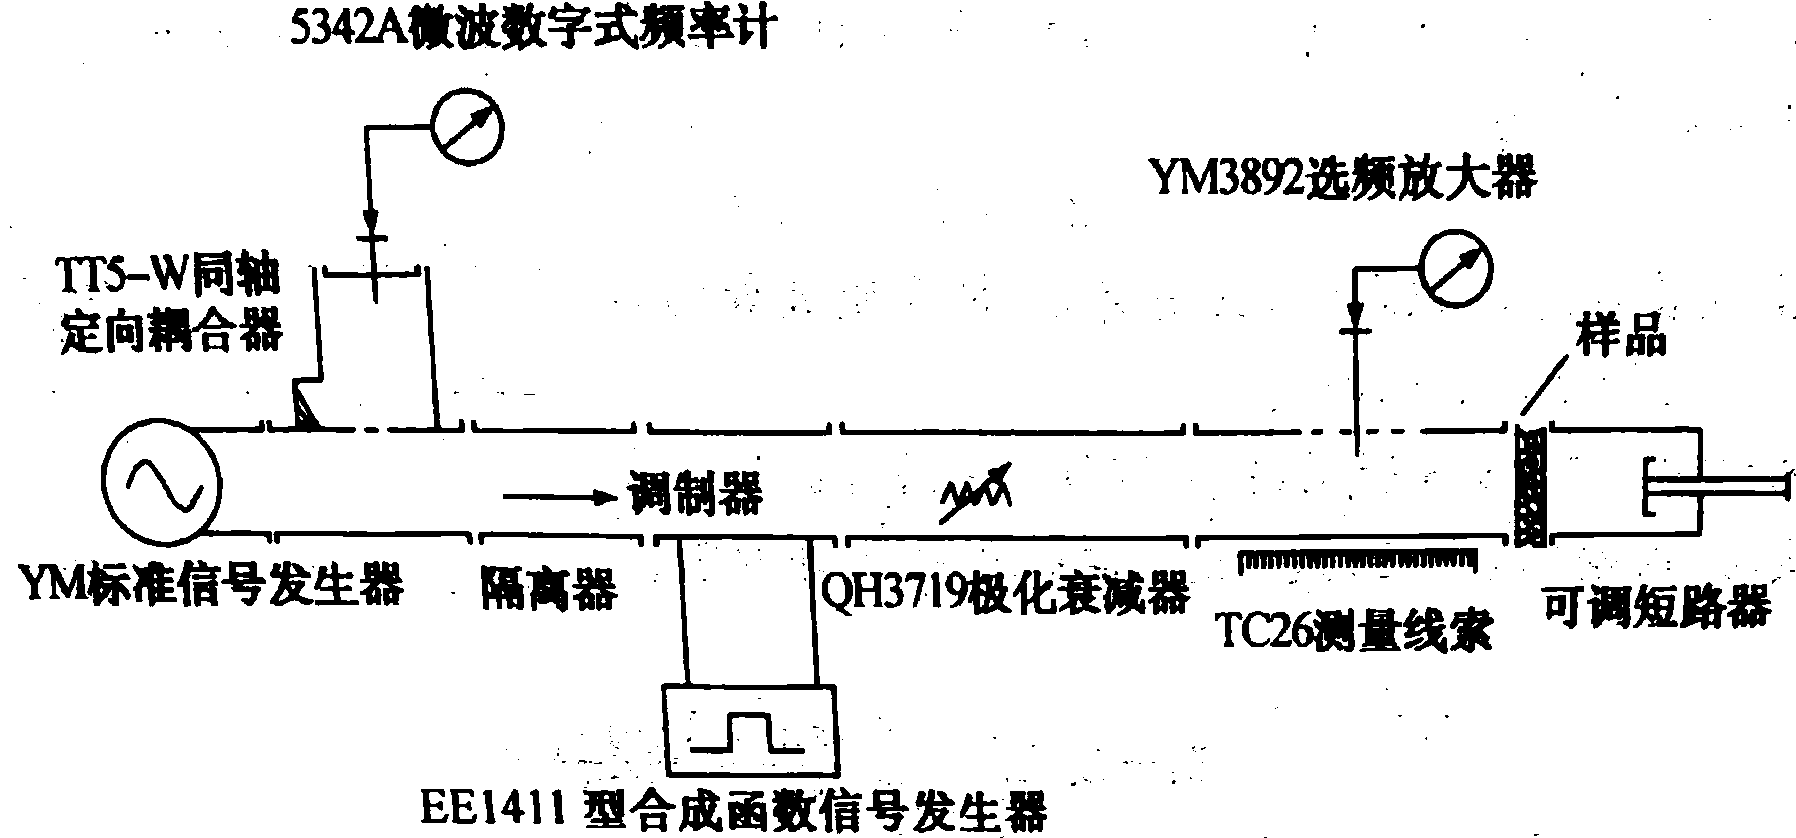
\includegraphics[width=0.8\textwidth]{fig/fig1.png}
	\caption{一种基于测量线的波导测量装置}\label{fig1}
\end{figure}

在微波测量中,是通过驻波的测量来得到阻抗。对图(\ref{fig1})所示的测量装置,可以用如图(\ref{fig2})所示的传输线模型进行分析。
\begin{figure}[!h]
	\centering
	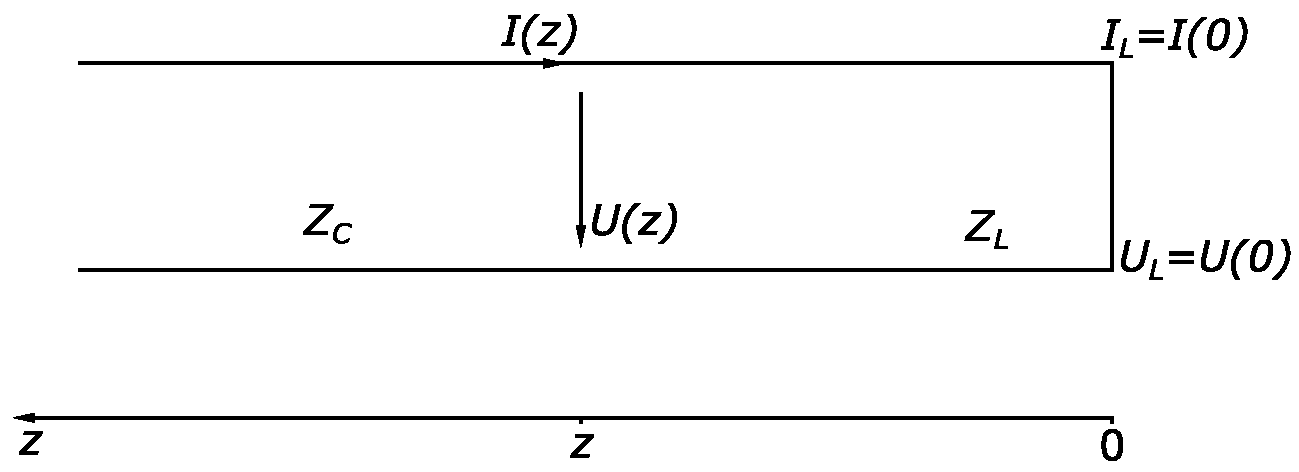
\includegraphics[width=0.8\textwidth]{fig/fig2.pdf}
	\caption{传输线模型}\label{fig2}
\end{figure}

以$e^{\gamma z}$表示入射波,$e^{-\gamma z}$表示反射波,$\gamma =\alpha + j\beta$为传播常数,入射波电压振幅与电流探幅之比为$+Z_C$,反射波此比值为$-Z_C$,坐标为$z$点的电压复振幅与电流复振幅之比称为该点输入阻抗,简称该点阻抗$Z(z)$,即:
\begin{equation}
	Z(z)=\frac{U(z)}{I(z)}=Z_C\frac{{\rm e}^{\gamma z}+\Gamma_L{\rm e}^{-\gamma z}}{{\rm e}^{\gamma z}-\Gamma_L{\rm e}^{-\gamma z}}=Z_C\frac{Z_L+Z_C\th(\gamma z)}{Z_C+Z_L\th(\gamma z)}\label{eq5}
\end{equation}

其中,$\Gamma_L$是负载上的电压反射系数,可以推得,
\begin{equation}
	\Gamma_L=\frac{Z_L-Z_C}{Z_L+Z_C}=|\Gamma_L|{\rm e}^{j\phi_L}\label{eq6}
\end{equation}

坐标为$z$点的电压反射系数为:
\begin{equation}
	\Gamma(z)=\frac{U_r(z)}{U_i(z)}=\frac{U_{rL}{\rm e}^{-\gamma z}}{U_{iL}{\rm e}^{+\gamma z}}=\Gamma_L\e^{-2\gamma z}=|\Gamma_L|\e^{-2\gamma z}\e^{-j(\phi_L-2\beta z)}=|\Gamma_L|\e^{j\phi(z)}\label{eq7}
\end{equation}

其中$|\Gamma (z)| = |\Gamma_L|e^{-2\alpha z}$,$\varphi (z) - \phi_L - -2\beta z$,于是从(\ref{eq5})式又推得:
\begin{equation}
	Z(z)=Z_C\frac{1+\Gamma_L(z)}{1-\Gamma_L(z)}\label{eq8}
\end{equation}

当线上有两点$Z_1$和$Z_2$,$Z_1 - Z_2 = l$,两点阻抗分别为$Z_1$,$Z_2$,则:
\begin{equation}
	Z_2=Z_C\frac{Z_1+Z_C\th(\gamma l)}{Z_C+Z_C\th(\gamma l)}\label{eq9}
\end{equation}

定义驻波最大点与最小点电压之比为电压驻波比:
\begin{equation}
	\rho=\frac{\e^{\gamma z_{\text{max}}}}{\e^{\gamma z_{\text{min}}}} \cdot\frac{1+|\Gamma(z_{\text{max}})|}{1-|\Gamma(z_{\text{min}})|}\label{eq10}
\end{equation}

在图(\ref{fig1})所示测量装置上,当终端短路时,即$Z_L = 0$,由(\ref{eq5})式知,样品输入端面向终端的等效阻抗为:
\begin{equation}
	Z_{1\text{短}}=Z_{C\text{介质}}\th(\gamma l_{\text{介质}})\label{eq11}
\end{equation}

$Z_1$也是空气波导的负载阻抗,其中$Z_{C\text{介质}}$是介质波导的特性阻抗,$l_{\text{介质}}$是测量样品的厚度。
\begin{figure}[!h]
	\centering
	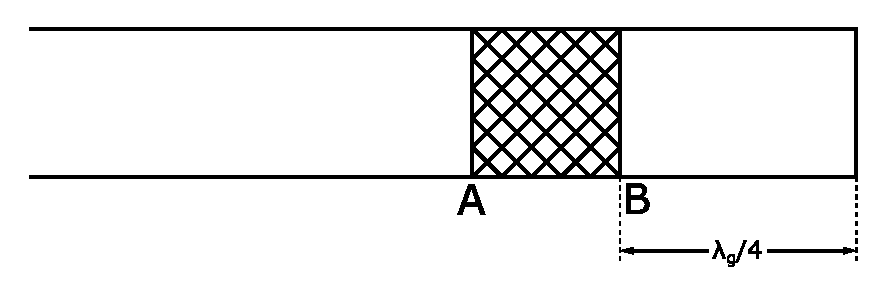
\includegraphics[width=0.8\textwidth]{fig/fig3.pdf}
	\caption{终端接入短路线示意图}\label{fig3}
\end{figure}

当终端如图(\ref{fig3})所示,接上四分之一波导波长长度的短路线时,根据(\ref{eq5})式,从B端向右看B处的阻抗为:
$$Z_B=Z_C\frac{Z_L+jZ_C\tan(k_g\lambda_g/4)}{Z_C+jZ_L\tan(k_g\lambda_g/4)}$$

此时$Z_L = 0$,$k_g = \frac{2\pi}{\lambda_g}$,因此$Z_B = Z_C\tan\frac{\pi}{2}\to\infty$,B端等效开路。于是,由(\ref{eq5})式知,样品输入端面向终端的等效阻抗为:
\begin{equation}
	Z_{1开}=Z_{C\text{介质}}\text{c}\th(\gamma l_{\text{介质}})\label{eq12}
\end{equation}

同时,由(\ref{eq5})式知,在距离样品输入端面D的驻波最小点处阻抗是:
$$Z(D)=Z_C\frac{Z_1+jZ_C\tan(k_gD)}{Z_C+jZ_1\tan(k_gD)}$$

由此得:
$$Z_1=Z_C\frac{1-j\frac{Z_C}{Z(D)}\tan(k_gD)}{\frac{Z_C}{Z(D)}-j\tan(k_gD)}$$

由(\ref{eq8})式得:
$$\frac{Z_C}{Z(D)}=\frac{1-\Gamma(D)}{1+\Gamma(D)}=\frac{1-|\Gamma|\e^{j\phi}}{1+|\Gamma|\e^{j\phi}}$$

在驻波最小点$e^{j\phi} = e^{j(2n+1)\pi} = -1$,所以
$$\frac{Z_C}{Z(D)}=\frac{1+|\Gamma|}{1-|\Gamma|}=\rho$$

由此得:
\begin{equation}
	\frac{Z_1}{Z_C}=\frac{1-j\rho\tan(k_gD)}{\rho-j\tan(k_gD)}\label{eq13}
\end{equation}

可见测出驻波比$\rho$即可得$\frac{Z_1}{Z_C}$。

对于柱状波导中的TE波,$Z_C = j\frac{\omega\mu}{\gamma}$,因此介质波导的$Z_{C\text{介质}} = j\frac{\omega\mu_0\mu_r}{\gamma}$,空气波导的$Z_C \approx \frac{\omega\mu_0}{k_g}$,因此,
\begin{equation}
	\mu_r=-j\frac{\lambda_g}{2\pi}\gamma\frac{Z_{C\text{介质}}}{Z_C}\label{eq14}
\end{equation}

由(\ref{eq11})式和(\ref{eq12})式得:
\begin{equation}
	\frac{Z_{C\text{介质}}}{Z_C}=\sqrt{\frac{Z_{1\text{短}}}{Z_C}\cdot\frac{Z_{1\text{开}}}{Z_C}}\label{eq15}
\end{equation}
\begin{equation}
	\gamma=\frac{1}{l_{\text{介质}}}\text{arc}\th\sqrt{\frac{Z_{1\text{短}}/Z_C}{Z_{\text{1开}}/Z_C}}\label{eq16}
\end{equation}

分别测出终端短路和等效开路两种状态的驻波比$\rho$,综合(\ref{eq13}),(\ref{eq14}),(\ref{eq15}),(\ref{eq16})式即可得到$\mu_r$值。

在介质波导中,
$$k_c^2=\omega^2\mu\epsilon+\gamma^2=k_0^2\mu_r\varepsilon_r+\gamma^2$$

因此,
\begin{equation}
	\varepsilon_r=\frac{k_c^2-\gamma^2}{k_0^2\mu_r} = \left(\frac{\lambda_0}{2\pi}\right)^2\frac{\left(\frac{2\pi}{\lambda_C}\right)^2 - \gamma^2}{\mu_r}\label{eq17}
\end{equation}

其中$\lambda_0$为自由空间波长,$\lambda_C$为波导截止波长。

从以上分析显见这种开路、短路两点法测量比较简便;可同时得到$\mu_r$和$\varepsilon_r$,且不需解超越方程。

\section{实验内容}
\begin{enumerate}
	\item 调节微波测试系统,选择好工作频率,测试系统处于稳定可靠的工作状态(极化衰减器置于0.5dB)。
	\item 测量待测材料厚度和波导板的厚度(用螺旋测微器,多点平均法)。
	\item 参考点位置的测量,测量线终端短路,用等指示法测得终端短路时最小点的位置作为参考点d。测量波导波长,与频率计测的频率计算出的波导波长比较误差。
	\item 短路测量材料参数。将材料片和短路板接入测量线的输出端,用等指示法测得最小点的位置和最小点的耦合电压放大值,用精密衰减器,用替代法测得电压最大值和最小值之间的替代分贝数。
	\item 开路测量材料参数。将可调短路活塞置于$\frac{\lambda_g}{4}$的位置使活塞波导口呈开路状态,与材料片一并接入测量线的输出端,与上相同测量开路状态下驻波最小点的位置最小点位置上耦合电压的放大值及与最大值的替代量。
	\item 用测得的数据输入程序计算出$\varepsilon_r$和$\mu_r$。
	\item 改变微波频率$f$,测量$\varepsilon_r$,$\mu_r$与频率$f$的关系。
\end{enumerate}

\section{注意事项}
\begin{enumerate}
	\item 先开微波源,在5$\sim$10分钟以后等幅微波频率信号才趋向稳定。
	\item 调节测量线的耦合输出和放大器的选频放大,在替代过程中放大倍数不变,每改变一个微波频率,测量线必须重新调谐耦合输出。
	\item 在开路测量中可调短路活塞的$\frac{\lambda_g}{4}$位置要保持不变。
\end{enumerate}

\section{实验数据}
首先,样品的厚度与波导的长度分别为:$\text{d} = 1.90\text{mm}$,$\alpha = 22.90\text{mm}$(前三个数据)、$\alpha = 15.6\text{mm}$(后三个数据),所以波导的截止波长分别为$\lambda_c = 2\alpha = 45.80\text{mm}$、$31.2\text{mm}$。根据公式
\begin{equation*}
	\lambda_g = \frac{\lambda}{\sqrt{1 - (\frac{\lambda}{\lambda_c})^2}}
\end{equation*}
可以计算理论波长$\lambda_{gT}$。

实验数据如表(\ref{table1:data})所示:
% Please add the following required packages to your document preamble:
% \usepackage{multirow}
% \usepackage[table,xcdraw]{xcolor}
% If you use beamer only pass "xcolor=table" option, i.e. \documentclass[xcolor=table]{beamer}
\begin{table}[!h]
	\begin{tabular}{|c|c|c|c|c|c|c|c|}
		\hline
		\multicolumn{2}{|c|}{$f$ / GHz}                               & 9                              & 10                            & 11                            & 12                            & 15                            & 17                                                          \\ \hline
		\multicolumn{2}{|c|}{$\lambda_{gT}$ / mm}                     & 48.61                          & 39.70                         & 33.95                         & 41.78                         & 26.06                         & 21.40                                                       \\ \hline
		\multicolumn{2}{|c|}{$\lambda_{gE}$ / mm}                     & 48.44                          & 39.58                         & 34.00                         & 40.80                         & 26.00                         & 21.10                                                       \\ \hline
		\rowcolor[HTML]{EFEFEF}
		\multicolumn{2}{|c|}{\cellcolor[HTML]{EFEFEF}$\lambda_g$误差} & -0.35\%                        & -0.30\%                       & 0.15\%                        & -2.34\%                       & -0.23\%                       & -1.4\%                                                      \\ \hline
		                                                              & Max / mV                       & 100(30dB)                     & 228(30dB)                     & 432(30dB)                     & 890(20dB)                     & 460(10dB)                     & 280(30dB)                   \\ \cline{2-8}
		                                                              & Min / mV                       & 260(50dB)                     & 510(50dB)                     & 100(40dB)                     & 140(30dB)                     & 660(30dB)                     & 70(40dB)                    \\ \cline{2-8}
		                                                              & \cellcolor[HTML]{EFEFEF}$\rho$ & \cellcolor[HTML]{EFEFEF}38.46 & \cellcolor[HTML]{EFEFEF}44.70 & \cellcolor[HTML]{EFEFEF}43.2  & \cellcolor[HTML]{EFEFEF}63.57 & \cellcolor[HTML]{EFEFEF}69.70 & \cellcolor[HTML]{EFEFEF}40  \\ \cline{2-8}
		\multirow{-4}{*}{短路}                                        & \cellcolor[HTML]{EFEFEF}D / mm & \cellcolor[HTML]{EFEFEF}96.50 & \cellcolor[HTML]{EFEFEF}74.20 & \cellcolor[HTML]{EFEFEF}93.70 & \cellcolor[HTML]{EFEFEF}3.2   & \cellcolor[HTML]{EFEFEF}2.4   & \cellcolor[HTML]{EFEFEF}1.6 \\ \hline
		                                                              & Max / mV                       & 115(dB)                       & 240(30dB)                     & 428(dB)                       & 360(dB)                       & 940(20dB)                     & 500(30dB)                   \\ \cline{2-8}
		                                                              & Min / mV                       & 160(50dB)                     & 490(dB)                       & 116(dB)                       & 460(dB)                       & 260(30dB)                     & 100(40dB)                   \\ \cline{2-8}
		                                                              & \cellcolor[HTML]{EFEFEF}$\rho$ & \cellcolor[HTML]{EFEFEF}71.88 & \cellcolor[HTML]{EFEFEF}48.98 & \cellcolor[HTML]{EFEFEF}36.90 & \cellcolor[HTML]{EFEFEF}78.26 & \cellcolor[HTML]{EFEFEF}36.15 & \cellcolor[HTML]{EFEFEF}50  \\ \cline{2-8}
		\multirow{-4}{*}{开路}                                        & \cellcolor[HTML]{EFEFEF}D / mm & \cellcolor[HTML]{EFEFEF}95.80 & \cellcolor[HTML]{EFEFEF}93.10 & \cellcolor[HTML]{EFEFEF}92.84 & \cellcolor[HTML]{EFEFEF}4.6   & \cellcolor[HTML]{EFEFEF}2.3   & \cellcolor[HTML]{EFEFEF}1.4 \\ \hline
	\end{tabular}
	\caption{实验数据}\label{table1:data}
\end{table}

代入上文的式(\ref{eq13}) $\sim$ (\ref{eq17})计算可得材料在不同频率下的相对磁导率和相对介电常数,如表(\ref{table2:mu_r and epsilon_r})所示:
\begin{table}[!h]
	\centering
	\begin{tabular}{|c|c|c|}
		\hline
		$f$ / GHz & $\mu_r$             & $\varepsilon_r$     \\ \hline
		9         & $0.2206-0.1378 i$   & $-13.8557+0.6376 i$ \\ \hline
		10        & $5.0619-0.2356 i$   & $-2.0827-0.0845 i$  \\ \hline
		11        & $38.8963-13.4231 i$ & $0.1531+0.0038 i$   \\ \hline
		12        & $-2.4930-0.1085 i$  & $1.7781-0.0297 i$   \\ \hline
		15        & $-2.9912+1.6825 i$  & $3.9948-2.8955 i$   \\ \hline
		17        & $-1.3018-1.3858 i$  & $4.3211+3.8696 i$   \\ \hline
	\end{tabular}
	\caption{相对磁导率$\mu_r$和相对介电常数$\varepsilon_r$}\label{table2:mu_r and epsilon_r}
\end{table}

将所得相对磁导率和相对介电常数的模值和相角与频率作图,如图(\ref{fig:data})所示:
\begin{figure}[!h]
	\centering
	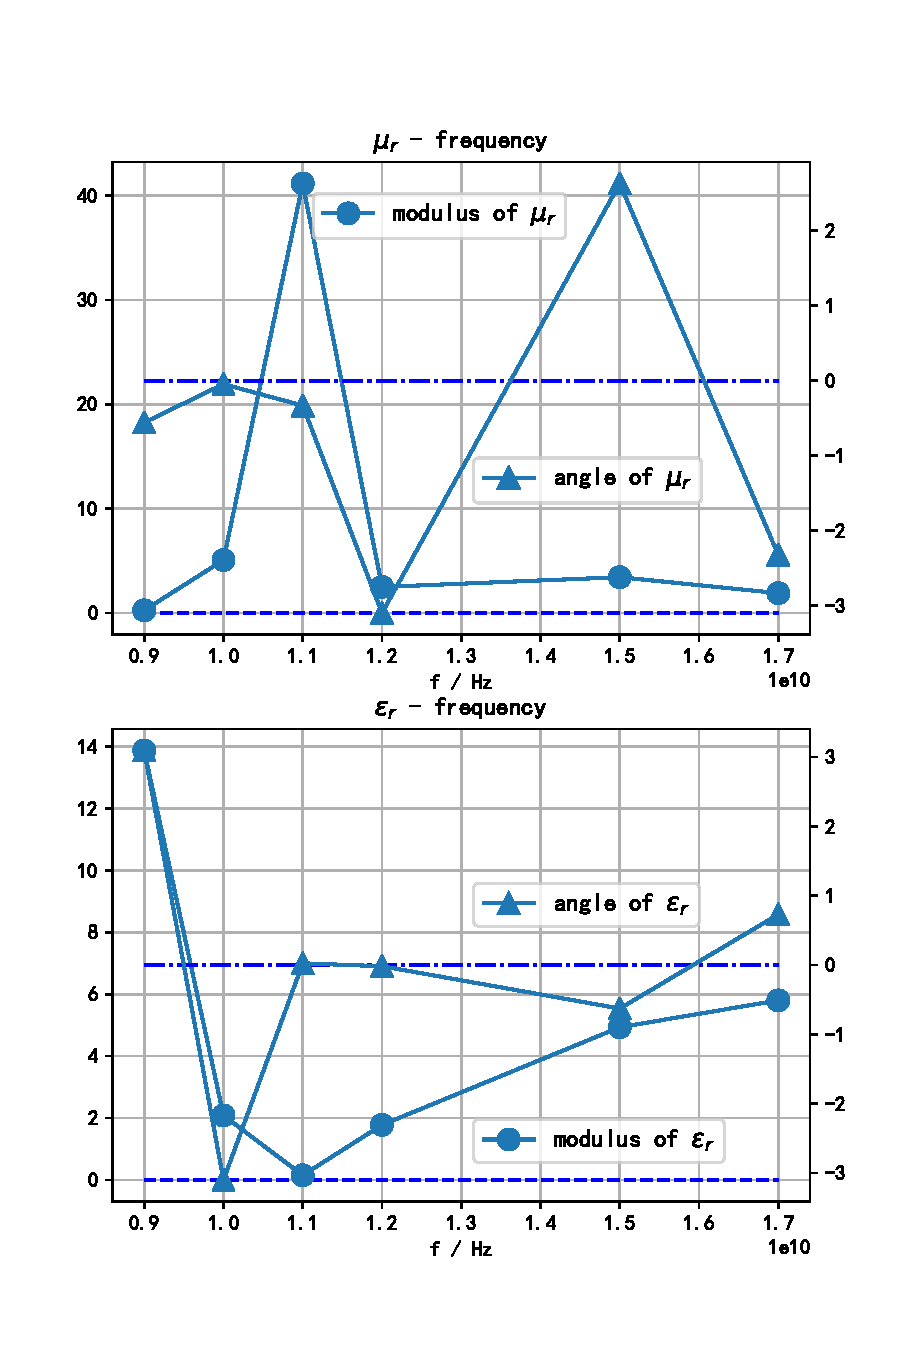
\includegraphics[width=0.7\textwidth]{fig/data.pdf}
	\caption{$\mu_r$、$\varepsilon_r$与频率$f$关系}\label{fig:data}
\end{figure}

\section{思考题}
\subsection{本实验测得材料的$\varepsilon$,$\mu$其主要误差来源是什么?}
\subsection{微波吸收材料要提高吸波性能,对$\varepsilon$,$\mu$有何要求?}

\nocite{jiaocai}
\bibliography{ref}
\end{document}